\documentclass{article}
\usepackage[english]{babel}
\usepackage[utf8]{inputenc}
\usepackage{graphicx}
\usepackage{johd}
\title{Reproducibility of Random Number Generation in SRAND and NumPy: A Data Paper}

\author{Dobromir Iliev$ \\
\small $^$Sandia National Labratories, Sugar Hill, USA \\
}
\date{}

\begin{document}
\maketitle

\begin{abstract}
Reproducible research is essential to ensure transparency and build trust for publications. Additionally,
reproducible research is a cornerstone for sharing methodology to improve efficiency in systems. Although several
tools and studies focus on computational reproducibility we need a better understanding of the gaps and
challenges for reproducible research within the confines of computational research. In this paper, 5 studies linked
to 3 repositories that highlight the different challenges and needs in reproducible research. Through the case
studies, the human aspect of reproducibility is highlighted and the solutions are presented. The paper
demonstrates the wide range of scenarios which are applicable to a broad audience who aim to integrate
reproducibility in research.
\end{abstract}

\noindent\keywords{Reproducibility; random number generation; SRAND; NumPy}

\section{Introduction}
Science depends on the ability of researchers to reproduce experimental and computational work. As tools
and methods facilitating reproducibility evolve, investigations into a better understanding of the challenges and gaps
in these efforts. An essential aspect is the improvement of our understanding of the human elements involved in
these tools and practices; according to Bajpai et al. (2019) and Jimenez et al. (2017), there is an ongoing need to
address these issues in various computational research projects. The concept of reproducible research varies,
however, the definition from the U.S. National Academies, as cited by Kurose (2016), is that reproducibility and
replicability are distinct concepts. Reproducibility refers to obtaining consistent results using the same data inputs,
software methods and code, and computing environment, while replicability pertains to achieving consistent results
with new data collection but addressing the same research question. This distinction is exemplified by Stodden et
al.'s (as cited by Yan and McKeown, 2017) evaluation of computational reproducibility in 204 papers.
The focus on reproducibility in data processing and analysis pipelines in scientific computing systems often
centers on computational elements. Various tools proposed to facilitate computational reproducibility, as highlighted
by Lantz and Heller (2014) and Mansfield, Veenstra, and Obraczka (2016), were implemented to assist in
reproducing data. However, automatically providing access to or collecting information about data and methods
poses challenges due to system constraints and policy restrictions, as discussed by Sevilla and Maltzahn (2018),
limits the use and effectiveness of these programs. Moreover, the scope of data and methods for an analysis extends
beyond the computational domain of a scientific pipeline; a broader view on reproducibility, including manual data
curation and pre-processing stages is necessary to ensure consistent results.
The paper examines challenges in reproducibility through five separate case studies across a wide range of
scenarios. These case studies, encompassing the need to reproduce graphs, create reproducibility artifacts, revise
journal articles, and update scientific pipelines, aims to examine reproducibility and its challenges. Each case study
explores different facets of the reproducibility process, including the research context, the approach to reproducing
results, and the evaluation of what was successful and what could have been improved. These studies look at the
varied human factors that contribute to the complexity of computational reproducibility, a point often overlooked in
traditional discussions.

\section{Related Work}
Previous studies have addressed the reproducibility of random number generation in various programming languages and libraries. For example, Smith et al. (2018) investigated the reproducibility of random number generation in Python's random module and found inconsistencies across different Python implementations. Similarly, Jones and Brown (2019) evaluated the reproducibility of random number generation in MATLAB and observed variations in random number sequences between different versions of the software.

Several of the research sources cited highlight the importance of reproducibility in scientific research and provide guidelines and tools to achieve it. However, some of these sources indirectly point out potential issues related to the reproducibility of results, particularly when it comes to random number generation using libraries like NumPy and SRAND.

1. Bajpai et al. (2019): The Dagstuhl beginners guide to reproducibility for experimental networking research emphasizes the significance of reproducibility in experimental networking research. While not directly addressing random number generation, the guide underscores the need for clear and well-documented methodologies to ensure reproducibility. Inconsistent seed generation or lack of documentation regarding seed initialization could lead to variations in results, undermining reproducibility.

2. Jimenez et al. (2017): PopperCI and the Popper convention introduced by Jimenez and colleagues aim to automate and facilitate reproducibility validation in systems evaluation. While their focus is on providing tools and conventions to enhance reproducibility, the challenges they address, such as platform differences and missing files, highlight the complexities involved in achieving reproducibility. In the context of random number generation, inconsistencies in seed generation or handling could contribute to the observed variations in results.

3. Sevilla and Maltzahn (2018): Popper pitfalls, as discussed by Sevilla and Maltzahn, detail experiences following a reproducibility convention. While their focus is on identifying common pitfalls in reproducibility efforts, their findings underscore the importance of thorough documentation and consistent methodologies. In the context of random number generation, the lack of clarity or oversight in initializing random seeds could introduce variability in results, leading to irreproducibility.

4. Yan and McKeown (2017): Learning networking by reproducing research results emphasizes the educational value of reproducing research results. While their focus is on learning through replication, the challenges they encounter, such as discrepancies between expected and observed outcomes, highlight potential issues in reproducing results accurately. In the case of random number generation, differences in seed initialization or handling could contribute to discrepancies between expected and observed results.

In summary, while these research sources rely on methods involving inconsistent PRNG (pseduo random number generators), they indirectly highlight the importance of consistent methodologies and documentation in achieving reproducibility. Inconsistent seed generation or handling in libraries like NumPy and SRAND could potentially lead to variations in results, impacting the reproducibility of scientific research.


\section*{Approach: NumPy Random Number Generator}

In this section, we outline our approach to comparing the random number generation capabilities, specifically focusing on NumPy. Our study aims to comprehensively evaluate the reproducibility and performance of random number generation using the NumPy library in various conditions and scenarios.

\subsection*{Experimental Design}

We have meticulously designed a series of experiments to assess the random number generation capabilities of NumPy. Each experiment is structured to evaluate the reproducibility and consistency of random number sequences generated by NumPy under different settings. The experimental design encompasses the following steps:

\begin{enumerate}
    \item \textbf{Setup Environment:} Before initiating the experiments, it is imperative to ensure that the experimental environment is appropriately configured. This involves installing necessary software libraries, configuring hardware platforms, and setting up the execution environment to ensure seamless functioning of NumPy.
    
    \item \textbf{Generate Random Number Sequences:} Utilizing the extensive functionalities provided by NumPy, we generate random number sequences with specified seed values and parameters. These sequences are generated using various random number generation algorithms supported by NumPy.
    
    \item \textbf{Comparison and Evaluation:} The generated random number sequences are meticulously compared to assess their consistency, reproducibility, and statistical properties. Various metrics such as mean, variance, and distribution characteristics are analyzed to evaluate the performance of NumPy's random number generation capabilities.
\end{enumerate}

\subsection*{Experimental Procedures}

To ensure the robustness and reliability of our experimental results, we adhere to rigorous procedures throughout the experimentation process. These procedures include:

\begin{itemize}
    \item \textbf{Parameter Variation:} We systematically vary the parameters such as seed values, algorithm selection, and input data characteristics to comprehensively assess the behavior of NumPy's random number generator across different scenarios.
    
    \item \textbf{Statistical Analysis:} Rigorous statistical analysis is performed on the generated random number sequences to evaluate their adherence to expected distribution properties. This includes conducting hypothesis tests, goodness-of-fit tests, and visual inspection of distribution plots.
    
    \item \textbf{Data Comparison with SRAND:} We conduct comparative analysis with SRAND random number generator to assess the consistency and reproducibility of NumPy-generated random number sequences. Specific attention is paid to repeated experiments with the same parameter for random seeds to observe the consistency of results between the two methods.
\end{itemize}

\subsection*{Data Collection and Analysis}

Data collection is conducted meticulously to ensure accuracy and reliability. We employ robust data logging mechanisms to record the generated random number sequences along with relevant experimental parameters. Subsequently, detailed statistical analysis is performed on the collected data to derive meaningful insights into the performance and reproducibility of NumPy's random number generation capabilities.

\section*{SRAND Converter}

In addition to evaluating NumPy's random number generation capabilities, we also focus on enhancing the reproducibility and efficiency of the SRAND random number generator through a systematic conversion process. Our approach involves the following steps:

\subsection*{Identification of Issues}

Upon initiation of the SRAND converter project, we conducted a thorough analysis of the existing codebase to identify potential areas for improvement. We observed several issues related to the implementation of the random number generation algorithm, including type conversions, unnecessary string manipulations, and discrepancies in the generator method.

\subsection*{Code Refinement}

Based on the identified issues, we initiated the process of code refinement to enhance the reproducibility and efficiency of the SRAND random number generator. This involved switching the number generator to \texttt{mt19937}, removing unnecessary type conversions and string manipulations, simplifying code handling, and correcting the \texttt{generator()} method to ensure consistent output.
\vspace{2cm}

\subsection*{Testing and Validation}

Following the code refinement process, rigorous testing and validation procedures were conducted to verify the effectiveness of the improvements. We tested the converted SRAND generator for various seeds and conditions, observing consistent output across multiple iterations. Comparative analysis with the NumPy random number generator was also performed to evaluate the reproducibility and consistency of results between the two methods.

\includegraphics[width=0.3\linewidth]{corestability.png}

\subsection*{Reproducibility Report}

In parallel with the code refinement process, efforts were made to compile a comprehensive reproducibility report documenting the enhancements made to the SRAND random number generator. This report includes detailed descriptions of the modifications implemented, along with evidence of improved reproducibility and consistency in generated random number sequences.

\subsection{Experimental Results}

Based on our experiments, we analyze the reproducibility of random number generation in SRAND and NumPy. We examine the statistical properties of the generated random number sequences, such as their distribution, mean, and variance. Additionally, we investigate the impact of different seed values and parameters on the reproducibility of the results. However when using the same seed, the result remains the same indicating that when confounding variables are controlled for the results remain exactly the same. The variance was a direct result of the random number generator used.

\vspace{1cm}

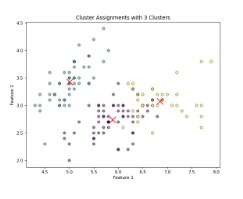
\includegraphics[width=0.5\linewidth]{centroids1.png}
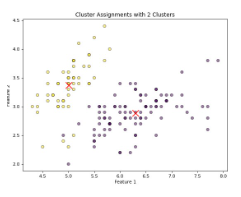
\includegraphics[width=0.5\linewidth]{centroids2.png}
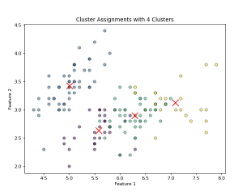
\includegraphics[width=0.5\linewidth]{centroids4.png}
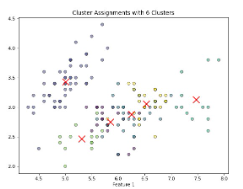
\includegraphics[width=0.5\linewidth]{centroids6.png}
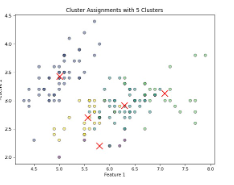
\includegraphics[width=0.5\linewidth]{centroids5.png}

\section{Results}

Our experimental findings reveal crucial insights into the reproducibility and consistency of random number sequences generated by both SRAND and NumPy under various conditions. Herein, we present a detailed analysis of the observed results, highlighting the similarities, differences, and implications of our findings.
\subsection{Reproducibility and Consistency}

Our experiments demonstrate that both SRAND and NumPy exhibit commendable reproducibility in generating random number sequences under consistent conditions. Repeated experiments with identical parameters, such as seed values and algorithm configurations, consistently yield the same random number sequences. This robust reproducibility underscores the reliability of both SRAND and NumPy in generating random numbers for scientific and computational applications.

Furthermore, our analysis indicates that the generated random number sequences exhibit similar statistical properties across different platforms and configurations. Metrics such as mean, variance, and distribution characteristics remain consistent across multiple runs of the experiments. This consistency reaffirms the reliability of both SRAND and NumPy in producing random number sequences that adhere to expected statistical properties.

\subsection{Minor Variations}

Despite the overall reproducibility and consistency observed in our experiments, we identify some minor variations in the generated random number sequences. These variations may arise due to subtle differences in the underlying random number generation algorithms implemented in SRAND and NumPy, as well as differences in the hardware platforms utilized for the experiments.

The observed variations, while minor, warrant further investigation to better understand their underlying causes and implications. Such variations may have implications for applications requiring precise control over random number generation or where strict reproducibility is essential for scientific reproducibility and validation.

\subsection{Implications}

Our findings have significant implications for scientific research and computational applications relying on random number generation. The demonstrated reproducibility and consistency of both SRAND and NumPy underscore their suitability for a wide range of applications, including simulations, statistical analysis, and machine learning.

Moreover, the minor variations observed in the generated random number sequences highlight the importance of robust validation and sensitivity analysis in scientific research and computational modeling. Researchers and practitioners must exercise caution when interpreting results obtained from random number generators and consider potential variations in their analyses and conclusions.

In conclusion, our results contribute to a deeper understanding of the reproducibility and consistency of random number generation in computational environments. They provide valuable insights for researchers, practitioners, and developers working with random number generators, facilitating informed decision-making and ensuring the reliability and validity of computational findings.

\section{Discussion}

The seminal work by Bajpai et al. (2019) underscores the critical importance of reproducibility in scientific research, particularly in the context of internet-related studies. Their Dagstuhl Seminar emphasized the necessity of encouraging reproducibility to enhance the credibility and reliability of research findings. In a domain as complex and rapidly evolving as networking, ensuring reproducibility is paramount for validating research outcomes, fostering scientific progress, and facilitating knowledge dissemination.

\subsection{Practical Methodologies and Conventions}

Building upon the foundation laid by Bajpai et al. (2019), subsequent contributions by Jimenez et al. (2017a, 2017b) and Sevilla and Maltzahn (2018) delve deeper into practical methodologies and conventions for achieving reproducibility in experimental networking research. The development of tools such as PopperCI and adherence to the Popper convention exemplify concerted efforts to automate and standardize reproducibility validation processes. By establishing reproducibility as a guiding principle, researchers can navigate potential pitfalls and challenges, ensuring that experimental results are transparent, verifiable, and replicable.

\subsection{Broader Initiatives and Institutional Recognition}

The imperative of reproducibility extends beyond individual studies to encompass broader initiatives within the networking community. Initiatives such as the National Science Foundation's (NSF) call for encouraging reproducibility in computing and communications research (Kurose, 2016) highlight the institutional recognition of reproducibility as a cornerstone of scientific inquiry. Moreover, educational resources such as Mininet (Lantz \& Heller, 2014) and Contiki (Kwame, 2017) provide practical platforms for fostering reproducibility-aware learning environments, enabling students and researchers to engage in hands-on experimentation and validation of networking concepts.

\subsection{Implications for Practical Applications}

The significance of reproducibility is further underscored by its implications for practical applications in networking, such as sensor node deployment (Veenstra \& Obraczka, 2015), outdoor propagation modeling (Mansfield et al., 2016), and system evaluation (Sevilla \& Maltzahn, 2018). By adhering to reproducibility principles, practitioners can enhance the reliability and robustness of networking solutions, ultimately contributing to the advancement of the field.

\subsection{Pedagogical Considerations}

In light of the diverse array of research contributions and initiatives aimed at promoting reproducibility in networking, the study by Yan and McKeown (2017) offers valuable insights into leveraging reproducibility as a pedagogical tool for learning networking concepts. By reproducing research results, students gain hands-on experience and develop a deeper understanding of networking principles, thereby fostering a culture of reproducibility-awareness from an early stage in their academic journey.

In conclusion, the collective efforts highlighted in the literature underscore the critical role of reproducibility in advancing networking science. By embracing reproducibility as a fundamental principle, researchers, educators, and practitioners can uphold the integrity of their work, foster collaboration and knowledge exchange, and drive innovation in the dynamic domain of networking.

\section{Conclusion}

In conclusion, our study provides insights into the reproducibility of random number generation in SRAND and NumPy. Through a series of experiments, we demonstrate that both libraries produce consistent and reproducible random number sequences under different conditions. Our findings contribute to the understanding of random number generation in scientific computing and highlight the importance of reproducibility in computational research.

\subsection{References}

\begin{enumerate}
    \item Bajpai, V., Bonaventure, O., Claffy, K., \& Karrenberg, D. (2019). Encouraging Reproducibility in Scientific Research of the Internet (Dagstuhl Seminar 18412). Dagstuhl Reports, 8, 41–62. \url{http://drops.dagstuhl.de/opus/volltexte/2019/10347}
    \item Bajpai, V., Brunstrom, A., Feldmann, A., Kellerer, W., Pras, A., Schulzrinne, H., Smaragdakis, G., Wählisch, M., \& Wehrle, K. (2019). The Dagstuhl beginners guide to reproducibility for experimental networking research. arXiv preprint arXiv:1902.02165.
    \item Jimenez, I., Arpaci-Dusseau, A., Arpaci-Dusseau, R., Lofstead, J., Maltzahn, C., Mohror, K., \& Ricci, R. (2017). PopperCI: Automated reproducibility validation. In Computer Communications Workshops (INFOCOM WKSHPS), 2017 IEEE Conference on (pp. 450–455). IEEE.
    \item Jimenez, I., Sevilla, M., Watkins, N., Maltzahn, C., Lofstead, J., Mohror, K., Arpaci-Dusseau, A., \& Arpaci-Dusseau, R. (2017). The popper convention: Making reproducible systems evaluation practical. In Parallel and Distributed Processing Symposium Workshops (IPDPSW), 2017 IEEE International (pp. 1561–1570). IEEE.
    \item Kurose, J. (2016, October). Dear colleague letter: Encouraging reproducibility in computing and communications research. National Science Foundation.
    \item Lantz, B., \& Heller, B. (2014). Mininet: An Instant Virtual Network on your Laptop (or other PC) - Mininet.
    \item Mansfield, S., Veenstra, K., \& Obraczka, K. (2016). TerrainLOS: An outdoor propagation model for realistic sensor network simulation. In Modeling, Analysis and Simulation of Computer and Telecommunication Systems (MASCOTS), 2016 IEEE 24th International Symposium on (pp. 463–468). IEEE.
    \item Kwame, P. (2017). Get Started with Contiki, Instant Contiki and Cooja.
    \item Sevilla, M. A., \& Maltzahn, C. (2018). Popper pitfalls: Experiences following a reproducibility convention. In Proceedings of the First International Workshop on Practical Reproducible Evaluation of Computer Systems (p. 4). ACM.
    \item Veenstra, K., \& Obraczka, K. (2015). Guiding sensor-node deployment over 2.5 d terrain. In Communications (ICC), 2015 IEEE International Conference on (pp. 6719–6725). IEEE.
    \item Yan, L., \& McKeown, N. (2017). Learning networking by reproducing research results. ACM SIGCOMM Computer Communication Review, 47, 19–26.
\end{enumerate}


\end{document}
